\documentclass[conference,letterpaper]{IEEEtran}
\usepackage[T1]{fontenc}
\usepackage{microtype}
\usepackage{amsmath,graphicx,booktabs,tabularx,array}
\usepackage[hidelinks]{hyperref}
\usepackage{url}
\renewcommand{\arraystretch}{1.12}
\setcounter{tocdepth}{2}
\emergencystretch=1em
\widowpenalty=10000
\clubpenalty=10000
\newcolumntype{Y}{>{\raggedright\arraybackslash}X}
% Generated from validated project inventories; run build_assets.py.
\newcommand{\NamedCount}{11,275}
\newcommand{\YesCount}{2,290}
\newcommand{\MaybeCount}{114}
\newcommand{\NoCount}{8,871}
\newcommand{\UntitledCount}{227}
\newcommand{\CategoryCount}{65}
\newcommand{\SlideCount}{83}
\newcommand{\TitleCount}{185}
\newcommand{\YesCategories}{32}
\newcommand{\MaybeCategories}{5}
\newcommand{\NoCategories}{28}
\newcommand{\BestHits}{54}
\newcommand{\StackHits}{51}
\newcommand{\BestPercent}{84.4}
\newcommand{\StackPercent}{79.7}

\title{Smithsonian Fossil Palynomorph Detection and Classification}
\author{\IEEEauthorblockN{Patrick Batsell, Yun Ying Tsai, Yeonju Kim, Yunfan Bao, and Alan Yang}
\IEEEauthorblockA{Rice University\\
Applied Machine Learning \& Data Science Projects\\
DSCI 435/535 \& COMP 449/549}}
\IEEEspecialpapernotice{Initial Report --- Fall 2026}

\begin{document}
% Course-specific front matter: a contents page and page numbers are required.
% The paper body uses the unmodified IEEE conference column layout.
\onecolumn
\maketitle
\thispagestyle{plain}
\pagestyle{plain}
\begin{center}
\textbf{Faculty Mentor:} Dr. Arko Barman, Rice University\\[3pt]
\textbf{PhD Mentor:} Nhi Le, Rice University\\[3pt]
\textbf{Sponsors:} Ingrid Romero and Scott Wing, Smithsonian Institution
\end{center}
\tableofcontents
\clearpage
\twocolumn

\section{Introduction}
\subsection{Problem and significance}
Pollen grains can survive in sediments long after the plants that produced them have disappeared. Identifying fossil pollen therefore gives researchers evidence about past vegetation. Smithsonian researchers aim to use this evidence to map North American plant distributions during the Eocene, a warm interval approximately 50 million years ago. These reconstructions can help assess whether climate simulations reproduce the conditions associated with ancient vegetation patterns \cite{proposal2026}.

The immediate challenge is collecting enough reliable identifications. A microscope slide can contain many specimens mixed with sediment and other organic material. An expert must locate each relevant grain, inspect its visible structures, and decide which category it belongs to. Repeating this process across a large collection is time-consuming. Digitized slides create an opportunity to automate parts of that work while allowing researchers to inspect the original images.

This project separates two tasks. \emph{Detection} identifies where a specimen is located; \emph{classification} assigns that specimen to a category. Previous Rice D2K work developed a whole-slide palynomorph detection workflow \cite{shaikh2026}. Our focus is to extend this foundation toward category identification and compare two ways of combining detection with classification. The intended application is a tool for expert-assisted analysis that supports subsequent studies of vegetation and climate.

\subsection{Objectives}
Our central question is whether fossil localization and category identification are better handled jointly by one detector or separately by a detector and a crop classifier. The project has four objectives:
\begin{enumerate}
\item Prepare a traceable dataset that connects each accepted specimen image to its original annotation, category, and source slide.
\item Compare a direct multiclass RF-DETR model with single-class RF-DETR followed by a Swin-Tiny classifier, using the same target categories and evaluation data.
\item Evaluate localization, category identification, and end-to-end performance, with attention to uncommon categories and changes in slide appearance.
\item Produce reusable code and a simple interface through which scientists can inspect specimens, candidate labels, and uncertain predictions.
\end{enumerate}
The category mapping and evaluation criteria will be specified before the main experiments.

\section{Background and Related Work}
\subsection{Pollen identification and multifocal imaging}
Palynomorphs are microscopic organic-walled particles, including pollen and spores. Identifying them can require distinguishing small differences in shape, pores or apertures, surface ornamentation, and wall structure. These features are not always visible in a single image plane. Multifocal scanning records the same region at several focal depths, allowing different parts of a specimen to come into focus \cite{shaikh2026,punyasena2022}.

For an image model, focal information presents a tradeoff. Selecting one sharp plane or combining sharp regions into a focus stack produces a two-dimensional input compatible with standard models. That compression can simplify processing but may remove depth-dependent information useful for classification. The initial comparison will use the same focus-stacked representation for both architectures. A later comparison with selected focal planes would be a separate experiment, using the same data partitions.

\subsection{Previous automated pollen identification}
Romero et al.\ \cite{romero2020} combined superresolution microscopy with convolutional neural networks to study fossil pollen taxonomy. They compared maximum-projection, multislice, and fused representations, training on modern pollen and applying the models to fossil specimens. Their study shows why image representation matters for taxonomic identification. It does not establish that conventional slide-scanner images will preserve the same diagnostic information.

Punyasena et al.\ \cite{punyasena2022} developed a two-stage detection and classification workflow for diverse Neotropical pollen samples. Their classification experiments considered 46 abundant taxa in an unevenly represented collection and examined how training objectives addressed that imbalance. This is a direct precedent for separating localization from identification. It motivates evaluating both stages and reporting category-level performance; the imaging conditions and biological categories differ from our fossil collection.

These studies establish that automated pollen identification is feasible in some settings. They do not remove the need to validate label definitions, image preparation, and generalization for this dataset. This study compares and integrates these approaches for the Smithsonian fossil collection.

\subsection{The existing whole-slide detection baseline}
Shaikh et al.\ \cite{shaikh2026} developed a scalable pipeline for fossil palynomorph detection in multifocal whole-slide images. The workflow divides large images into overlapping tiles, compresses focal information, applies an object detector, and merges duplicate predictions in slide coordinates. Its reported detection study used 82 annotated slides drawn from a collection of 847 slides. The present classification dataset contains \SlideCount{} annotated slides.

The paper reports average precision of 0.879 at an intersection-over-union threshold of 0.50 for its strongest RF-DETR configuration, and optimized whole-slide inference in under one hour on its reported setup. These published detection results motivate evaluating the framework for category identification. Their work supplies a practical starting point for image handling and localization. Adding category identification introduces different requirements for annotation consistency and preservation of specimen morphology.

\subsection{Motivation for the proposed architectures}
Roboflow Detection Transformer (RF-DETR) is a transformer-based object detector designed for transfer to target datasets \cite{robinson2026}. It is a suitable baseline here because it was evaluated in the preceding palynomorph study and can jointly output locations and categories. The model variant, software version, and pretrained checkpoint will be fixed and recorded before training.

Swin Transformer builds hierarchical image representations with attention within local windows and connections across shifted windows \cite{liu2021}. We propose its small Swin-Tiny variant as the crop classifier. Processing a centered specimen could help the model focus on morphology, but that is a hypothesis to test. Neither Swin's general vision results nor its architecture demonstrates an advantage over a joint detector on these fossils.

\section{Data and Initial Exploration}
\subsection{Sources and file structure}
The dataset comprises \SlideCount{} digitized microscope slides with paired expert annotations. Images are stored as NanoZoomer Digital Pathology Image (NDPI) files; separate NanoZoomer Digital Pathology Annotation (NDPA) files contain annotation titles and geometry. The images are accessed through Rice's NOTS computing system \cite{inventory2026}.

The data must be considered at several levels: a source slide, its image regions and focal planes, and the annotated specimens within those regions. Multiple focal planes or overlapping crops of one specimen are related observations, not independent examples. Each derived crop will retain its slide identifier, annotation identifier, coordinates, original title, and mapped category.

Annotation titles are mapped to categories using the expert-provided label tables. These categories include both finer taxonomic identifications and broader biological or morphological groups. Broader groupings may be evaluated before finer category distinctions.

The dataset contains \NamedCount{} named annotation records representing \TitleCount{} annotation titles mapped to \CategoryCount{} categories. Of these, \YesCount{} records across \YesCategories{} categories form the initial classification inventory. Table~\ref{tab:inventory} summarizes category-selection priorities \cite{inventory2026}.

\begin{table*}[t]
\centering
\caption{Annotation inventory and category-selection priorities. Counts precede crop-quality checks, duplicate review, broad-category grouping, and training sampling.}
\label{tab:inventory}
\begin{tabularx}{\linewidth}{lrrY}
\toprule
Selection priority & Categories & Records & Initial treatment \\
\midrule
YES & \YesCategories & \YesCount & Starting inventory for category classification \\
MAYBE & \MaybeCategories & \MaybeCount & Retain separately pending inclusion decisions \\
NO & \NoCategories & \NoCount & Outside the initial target-category selection \\
\midrule
Named total & \CategoryCount & \NamedCount & Complete named inventory \\
Untitled & --- & \UntitledCount & Not assigned category labels \\
\bottomrule
\end{tabularx}
\end{table*}

The \UntitledCount{} untitled marks include 133 rectangles and 94 circles. They are excluded from named category counts. In particular, the \YesCount{} YES records are an annotated starting inventory, not a finalized set of unique, quality-checked training specimens.

The YES, MAYBE, and NO designations indicate category-selection priorities rather than specimen presence or label confidence. Excluded categories can still contain palynomorphs; consequently, these records and unannotated regions require separate treatment from confirmed background in detection experiments.

\subsection{Class balance and coverage across slides}
Figure~\ref{fig:counts} shows the \YesCategories{} inclusion-priority categories before regrouping or sampling. Counts range from 27 for Cupuliferoipollenites sp.\ to 316 for Bisaccate. The number of slides represented also varies. Retipollenites sp.\ has 75 records on only three slides, with 72 on one slide. A large annotation count can therefore conceal limited independent coverage \cite{inventory2026}.

Three categories of particular scientific interest are Arecipites sp.\ (81 records on 20 slides), Bombacacidites sp.\ (40 on 17), and Platycarya platycarioides (56 on six). Their coverage will be reported explicitly during data preparation and evaluation. We will preserve the original fine labels even if the initial training task uses broader groups.

\begin{figure*}[t]
\centering
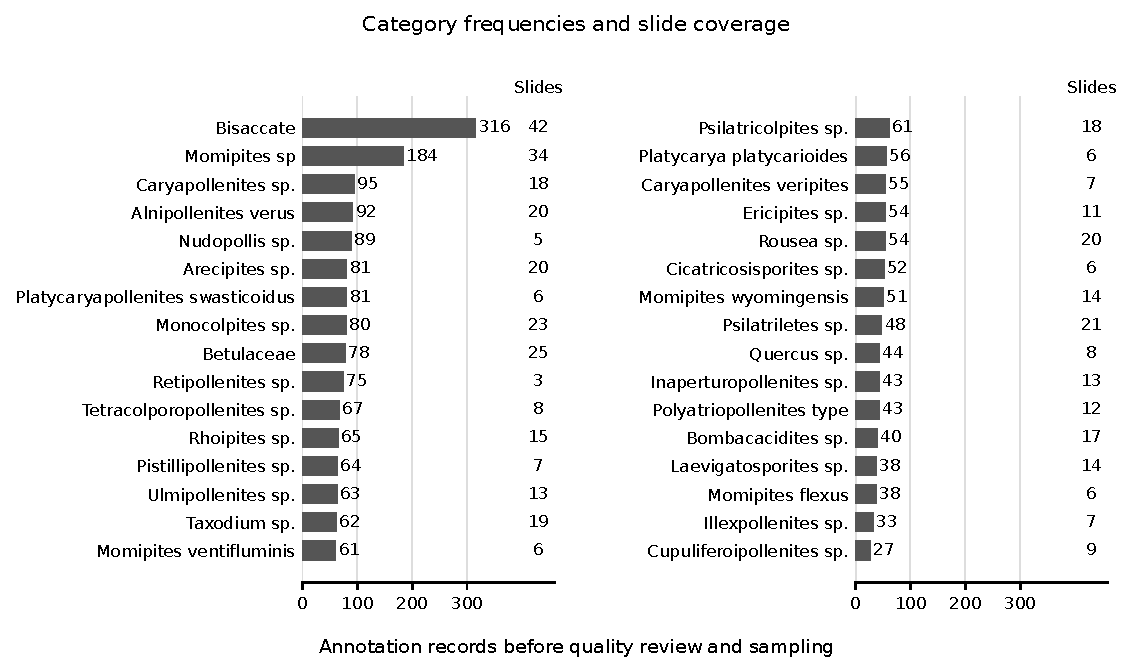
\includegraphics[width=\linewidth]{figures/category_distribution.pdf}
\caption{Annotation counts and slide coverage for all 32 inclusion-priority categories in the dataset. Bar lengths show annotation records; the right column gives the number of slides containing each category. These are source counts, not final training sizes or estimates of biological abundance. Counts are derived from the annotation inventory \cite{inventory2026}.}
\label{fig:counts}
\end{figure*}

Uneven representation motivates per-class evaluation and comparison of training strategies. Candidate approaches include random undersampling of abundant categories, class-balanced sampling within training batches, and class-weighted loss functions that give greater weight to underrepresented categories. Undersampling can reduce imbalance but discards potentially useful examples; repeated sampling of rare categories does not add biological diversity. These strategies can be compared with training on all available training examples under a fixed validation split. All balancing will be confined to training, with validation and test distributions held fixed.

\subsection{Data quality and remaining preparation}
Image-quality assessment will examine coordinate alignment, focus, duplicate specimens, and category assignments. Boxes derived from expert circles may contain more surrounding space than tight detector boxes, affecting overlap scores. Annotations are not established as exhaustive whole-slide labels. Regions used to measure false positives will need a completeness review.


Figure~\ref{fig:specimens} illustrates variation in morphology, staining, and surrounding material across expert-labeled specimens.

\begin{figure*}[t]
\centering
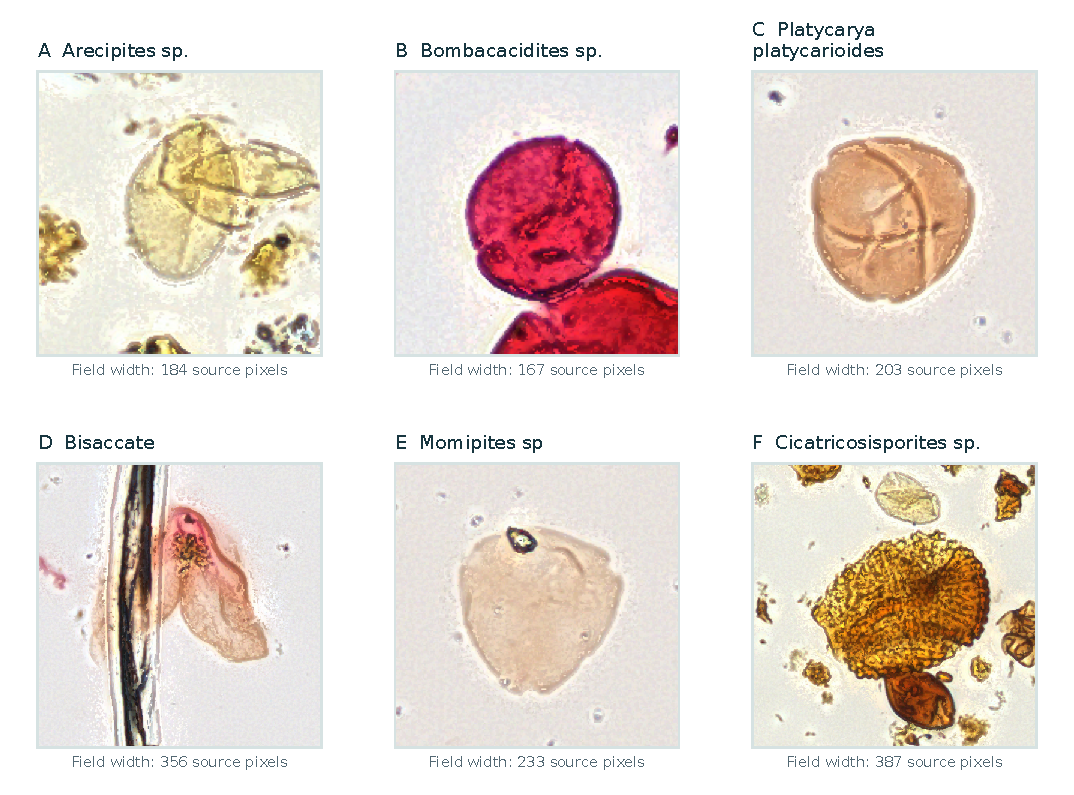
\includegraphics[width=\linewidth]{figures/specimen_examples.pdf}
\caption{Expert-labeled palynomorph examples from focus-stacked images. A--C show three categories of particular scientific interest; D--F illustrate additional morphology and surrounding material. Labels refer to the annotated central specimen. Crops retain the original focus-stacked pixel values. Field widths are given in source pixels and differ between panels; displayed sizes do not indicate relative physical size.}
\label{fig:specimens}
\end{figure*}

\section{Data Science Pipeline}
\subsection{Annotation checks and specimen extraction}
Each annotation will be linked to its corresponding image, and its physical coordinates will be converted to pixel coordinates using the image metadata. Horizontal and vertical pixel sizes will be handled separately. A small inspection batch will cover multiple categories, focal planes, slide boundaries, and specimens outside historical training rectangles.

Accepted crops will preserve the original annotation and record the derived bounding box, extraction settings, and any exclusion reason. The final category mapping will be versioned separately from the original labels. Uncertain identifications and categories outside the initial task will remain identifiable instead of being silently reassigned.

For detector inputs, large images will be processed as overlapping tiles with a fixed size and overlap. Focus stacking will combine information across focal planes into a two-dimensional image. For classifier inputs, accepted specimen boxes will define crops with a fixed surrounding margin. The exact tiling, focus-stacking, and margin settings will be selected during preparation and held constant across the main comparison.

\subsection{Partitioning and training preparation}
Training, validation, and test groups will be assigned before tiling, augmentation, or class balancing. At minimum, all specimens from a source slide will remain in one partition. Metadata will also be checked for shared geological samples or preparations that require grouping multiple slides together. All focal planes, overlapping views, and augmented versions of a specimen will follow its assigned group.

Split proportions or grouped folds will be chosen after examining category coverage across independent groups. The final test set will remain unused during model and threshold selection. Historical training membership of any reused detector checkpoint must also be reviewed: a newly assigned test slide is not independently held out if that checkpoint was previously trained on it.

Both proposed approaches will use the same approved categories and eligible source material. A common set of reviewed detector-training regions will be established so that differences in missing labels do not favor one model. Regions that contain unlabeled target objects cannot simply be treated as fully annotated negatives. Any augmentation, normalization, class weighting, or sampling will be documented and fitted or applied using training data only.

\subsection{Prediction output and expert review}
At inference, tile predictions will be mapped to whole-slide coordinates and duplicates merged. Outputs will retain a specimen's location, predicted category, model scores, and source image identity. The planned viewer will let a researcher inspect the specimen and alternative labels, with access to focal planes where available.

Uncertainty thresholds and the handling of specimens outside the trained categories remain open. A classifier restricted to a fixed set of categories can assign a confident label to an unfamiliar object. Until rejection behavior has been evaluated, the interface will present scores as model outputs for review, not as calibrated probabilities of biological correctness. Original expert annotations will remain separate from generated predictions.

\section{Proposed Models}
We use the RF-DETR-based detection workflow of Shaikh et al.\ \cite{shaikh2026} as the baseline. Both proposed approaches extend localization to category identification and will use the same approved category set, source groups, focus-stacked inputs, and held-out evaluation regions. Let $K$ denote the number of final target categories; it is not yet fixed to the 32 inclusion-priority categories.

\subsection{Model 1: Direct multiclass RF-DETR}
The first approach extends the single-class detector to jointly predict each specimen's location and category. Given an image $I$, it produces a set of predictions
\[
\widehat{Y}=\{(\widehat{b}_i,\widehat{c}_i,\widehat{p}_i)\}_{i=1}^{N},
\]
where $\widehat{b}_i$ is a bounding box, $\widehat{c}_i$ is a category, and $\widehat{p}_i$ is the associated model confidence score. The inference workflow is shown in Figure~\ref{fig:model1}.

\begin{figure*}[t]
\centering
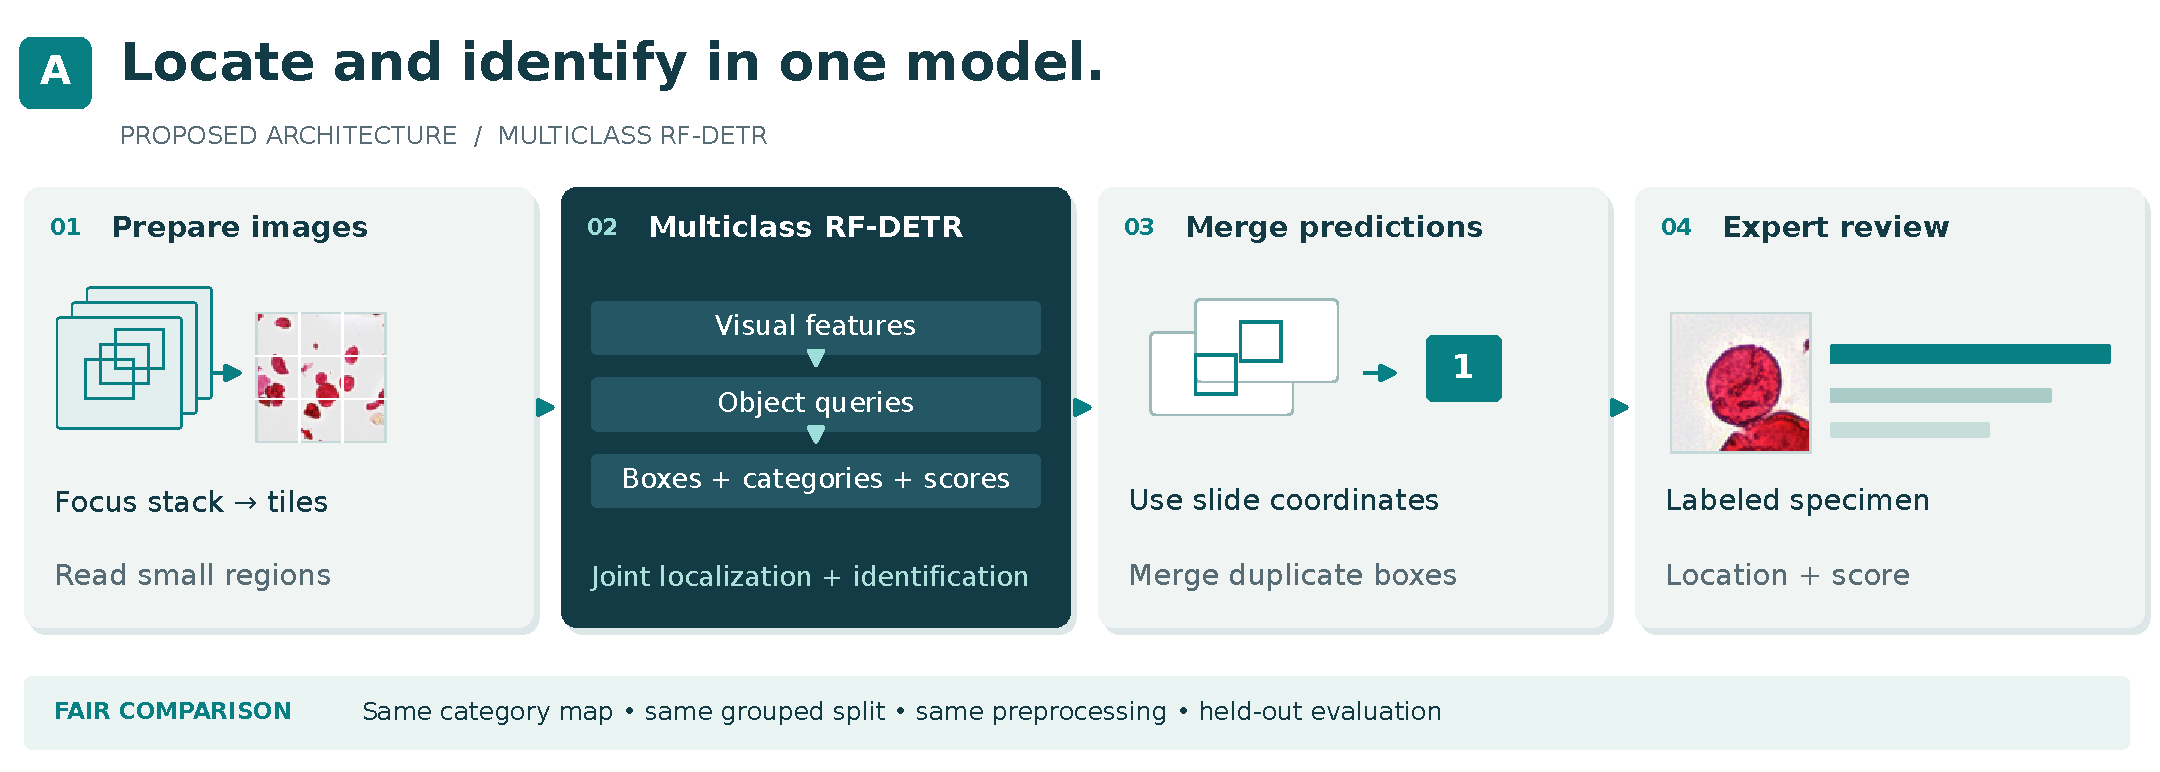
\includegraphics[width=\linewidth]{figures/workflow_direct.pdf}
\caption{Proposed multiclass RF-DETR architecture. Overlapping image tiles are processed jointly for localization and category identification, then predictions are merged in slide coordinates. Model modules and output indicators are schematic; thumbnails show focus-stacked specimen images.}
\label{fig:model1}
\end{figure*}

Each training box will be associated with an approved category and source group. RF-DETR will be initialized from a compatible pretrained checkpoint, and its classification output will be adapted to the $K$ target categories. The model will then be fine-tuned on the training partition. Validation data will guide checkpoint selection, training settings, and confidence thresholds.

During inference, predictions from overlapping tiles will be mapped back to slide coordinates. A documented duplicate-merging rule will produce the final specimen list. Disagreements between overlapping category predictions will be resolved using a rule fixed on validation data and then applied unchanged to the test set.

The primary advantage is a single model that learns localization and category identification together. A possible limitation is that rare or visually similar categories may be difficult to learn within the joint objective. Localization and category errors will therefore be analyzed separately where the matching between predictions and annotated specimens permits it.

\subsection{Model 2: RF-DETR with Swin-Tiny classification}
The second approach separates localization from category identification. RF-DETR will detect eligible specimens as one object class, after which Swin-Tiny will classify a crop of each detection. Figure~\ref{fig:model2} includes both tile aggregation and classification so that duplicate tile detections are not counted as independent specimens.

\begin{figure*}[t]
\centering
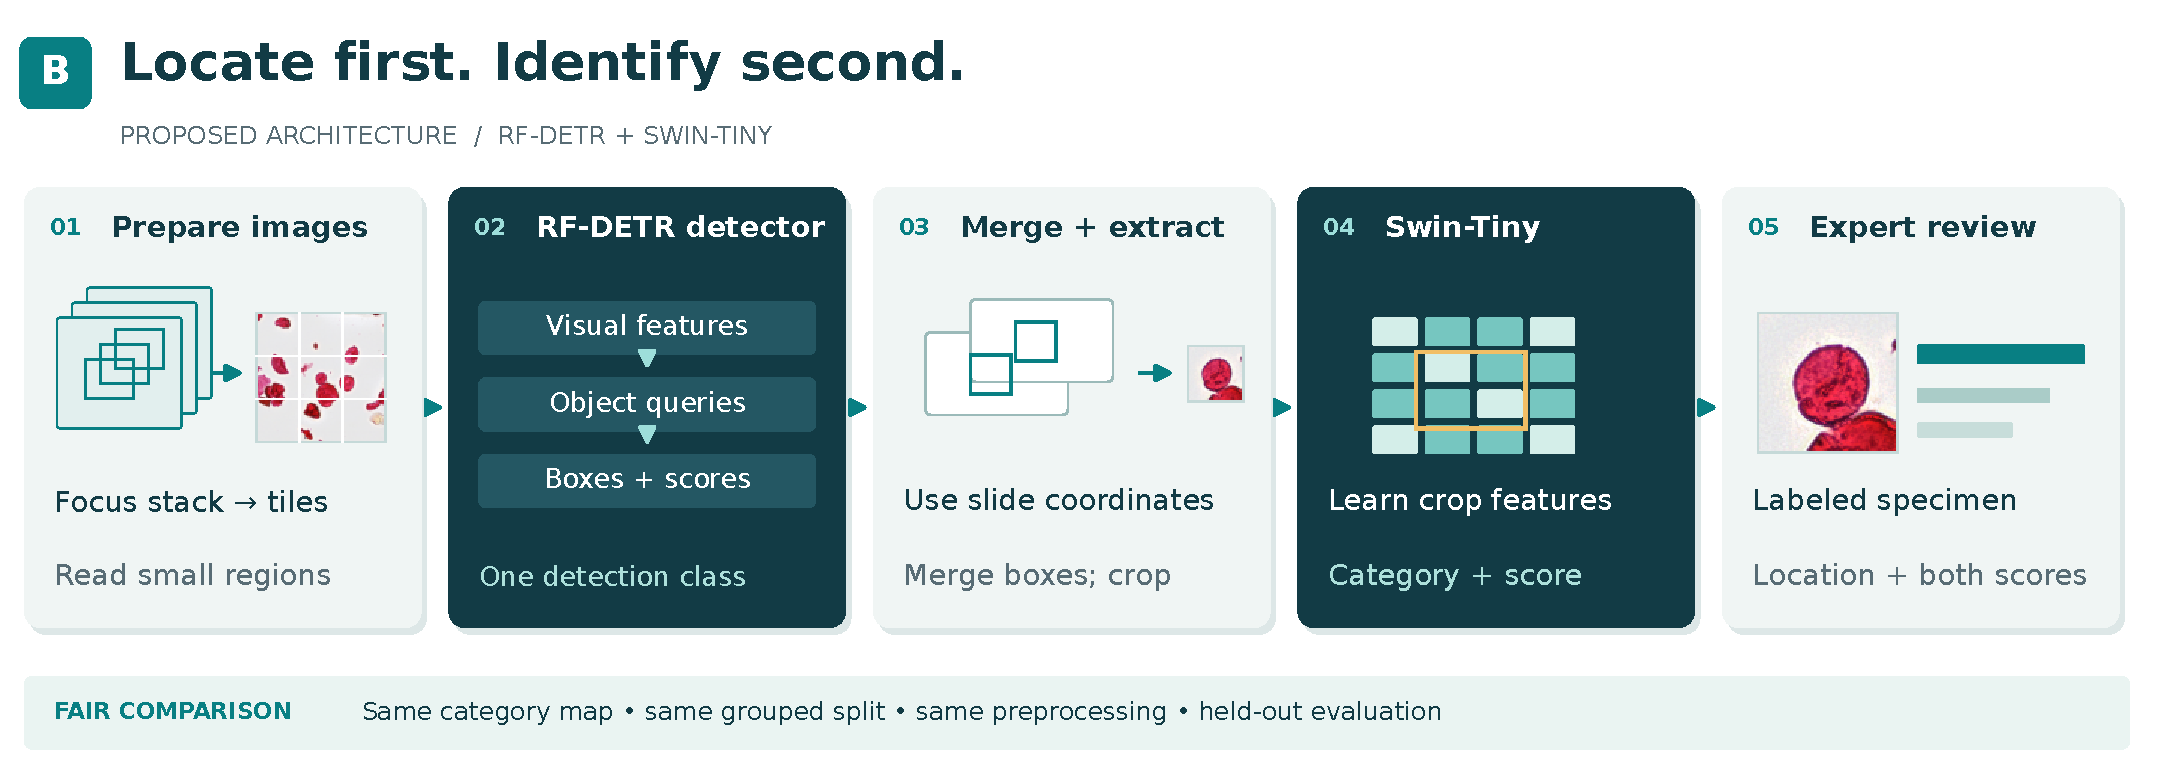
\includegraphics[width=\linewidth]{figures/workflow_two_stage.pdf}
\caption{Proposed two-stage architecture. RF-DETR localizes specimens; merged detections define crops for Swin-Tiny classification. Detector and classifier scores are retained separately. Model modules and output indicators are schematic; thumbnails show focus-stacked specimen images.}
\label{fig:model2}
\end{figure*}

\subsubsection{Stage 1: Palynomorph detection}
For the controlled comparison, category annotations for eligible target specimens will be collapsed into a single detection class. The detector will use the same reviewed regions and group split as Model 1. The broader historical palynomorph detector is a reference baseline; it will not be assumed to have the same target definition or training exposure.

Recall will be important when selecting a detector operating threshold because missed specimens cannot be recovered by the second stage. However, lowering the threshold also produces more candidate crops, including false detections. Threshold selection will therefore consider downstream performance and review workload on validation data.

\subsubsection{Stage 2: Swin-Tiny classification}
Initial classifier training crops will come from expert annotations rather than detector predictions. After checking annotation geometry, each crop will include a fixed margin, be padded to a square, and be resized to $224\times224$ pixels without changing its aspect ratio. The initial input resolution will be assessed for preservation of diagnostic morphological detail.

Swin-Tiny will be initialized from pretrained weights, with its final output layer replaced by a $K$-category classifier. Its hierarchical shifted-window attention provides a way to learn local and broader image features \cite{liu2021}. The working hypothesis is that a centered crop may make category-specific morphology easier to learn than it is in a larger detection tile.

At inference, crops from RF-DETR boxes will use the same margin, padding, and resizing procedure. Detector and classifier scores will initially be retained separately. Any rule used to combine them for ranking end-to-end predictions will be specified and fixed using validation data before test evaluation.

The main advantage is that classification can be assessed independently on expert crops, making error analysis more direct. The main limitation is error propagation: an undetected specimen is unavailable to the classifier, and an incomplete or inaccurate crop can remove diagnostic features. Training on expert crops may also differ from deployment on predicted crops. Both settings will therefore be evaluated explicitly.

\subsection{Comparison and modeling assumptions}
Table~\ref{tab:models} summarizes the comparison. The same source data and evaluation rules will be used, but the approaches have different computational requirements. The comparison is intended to assess useful system performance, not to claim that the two architectures have identical parameter counts or training costs.

\begin{table*}[t]
\centering
\caption{Proposed model comparison. Both systems predict specimen locations and categories; their division of the task differs.}
\label{tab:models}
\begin{tabularx}{\linewidth}{p{0.20\linewidth}YY}
\toprule
Dimension & Model 1: Multiclass RF-DETR & Model 2: RF-DETR + Swin-Tiny \\
\midrule
Strategy & Joint localization and classification & Detection followed by crop classification \\
Main advantage & One model and a unified inference stage & Independent classifier evaluation and specimen-focused inputs \\
Key dependency & Reliable category labels for detector training boxes & Reliable detections and category-labeled crops \\
Likely failure & Confusion among rare or similar categories & Missed specimens and poor crops propagate downstream \\
Main question & Can one detector learn both tasks effectively? & Does separate crop classification improve identification? \\
\bottomrule
\end{tabularx}
\end{table*}

The comparison assumes a consistent category mapping, usable annotation geometry, and sufficient independent groups for evaluation. These assumptions will be checked before training. The broad-category mapping, treatment of uncertain or excluded specimens, model sizes, and detailed training settings remain unresolved. They will be documented before the main comparison rather than selected in response to test results.

\subsection{Model evaluation}
\subsubsection{Localization and end-to-end detection}
Intersection over union (IoU) measures the overlap between a predicted box and a reference box: intersection area divided by union area. On sufficiently complete, reviewed evaluation regions, we will report Average Precision at IoU 0.50 ($\mathrm{AP}_{50}$) and mean Average Precision across IoU thresholds 0.50 to 0.95 in increments of 0.05 ($\mathrm{AP}_{50:95}$). Precision measures the fraction of reported detections that are correct; recall measures the fraction of reference specimens recovered.

Class-agnostic localization will be compared on a common eligible target set. End-to-end evaluation will use multiclass AP and correctly classified specimen recall, requiring both a matched location and the correct category. One-to-one matching and tile deduplication will prevent repeated detections from receiving repeated credit. The original single-class baseline will only be compared where target definitions and checkpoint exposure allow a meaningful interpretation.

These precision and AP measures require reliable knowledge of which predictions are false positives. If a region is incompletely labeled, unmatched predictions cannot automatically count as errors. Establishing an exhaustively reviewed evaluation subset is therefore a prerequisite for those claims. Recovery of known annotated positives will be reported separately when complete labels are unavailable.

\subsubsection{Category identification and error analysis}
For classification, we will report macro-F1, balanced accuracy, per-class precision and recall, and a confusion matrix. Macro-F1 gives each evaluated category equal weight when averaging its precision--recall summary. Balanced accuracy averages class recall. These measures complement overall accuracy when category frequencies differ. Each result will include the number of reference specimens and source groups; categories absent from an evaluation partition will be disclosed.

Swin-Tiny will first be evaluated on crops derived from held-out expert annotations. It will then be evaluated on matched detector crops to assess sensitivity to crop quality. Classification results on detected specimens alone will be labeled as conditional on detection; the end-to-end recall calculation will still count missed specimens as failures. Errors will be reviewed for category confusion, focus, preservation, staining, bounding-box quality, and slide-specific patterns.

The comparison will also report whole-slide inference time, peak memory use, hardware, and preprocessing settings. Uncertainty estimates should respect the grouped data: resampling will operate on independent slide or sample groups rather than treating all crops as independent. If too few independent groups are available, the report will state that limitation instead of presenting precise-looking estimates unsupported by the data.

\subsubsection{Reliability and reproducibility}
Source checksums, the category map, specimen identities, split assignments, preprocessing, code versions, model checkpoints, training settings, and random seeds will be recorded for each experiment. Model and threshold selection will use validation data. The test set will be used for the final comparison after the protocol is fixed. A small example will demonstrate how the pipeline processes previously unseen data with the same settings.

\section{Preliminary Detector Assessment}
A preliminary detector assessment evaluates the feasibility of reusing existing checkpoints on the labeled collection. It does not evaluate the proposed classification models; final category grouping, specimen-quality assessment, and the experimental split remain prerequisites for that comparison.

The assessment tested two pretrained, frozen You Only Look Once (YOLO) checkpoints on 64 annotated targets from 29 slides, with two targets per inclusion-priority category. Each target was placed in a $1024\times1024$ image region. A target counted as recovered when a predicted box had confidence at least 0.50 and IoU at least 0.50. Table~\ref{tab:pilot} summarizes the results \cite{pilot2026}.

\begin{table}[htbp]
\centering
\caption{Existing annotation-centered detector diagnostic, not a test of the proposed classification models. Each row uses a different frozen YOLO checkpoint.}
\label{tab:pilot}
\begin{tabular}{lrr}
\toprule
Input & Recovered & Proportion \\
\midrule
Best focal plane & \BestHits/64 & \BestPercent\% \\
Focus stack & \StackHits/64 & \StackPercent\% \\
\bottomrule
\end{tabular}
\end{table}

This diagnostic establishes that the existing software and weights can process the sampled image regions and recover many of their known targets. It does not estimate whole-slide precision, AP, or category-classification accuracy. Targets were centered rather than encountered through blind tiling, and two examples per category are insufficient to estimate category performance. Because the checkpoints differ, the comparison also does not isolate the effect of focal preprocessing.

Historical split records list 50 targets on training slides, nine on test slides, and five with unresolved membership. Those records are not fully verified checkpoint provenance, so independent generalization cannot be inferred. One inspected failure also illustrates a box-convention issue: a tight predicted box can have insufficient overlap with a larger square derived from an annotation circle. These cases motivate reviewing annotation-to-box conversion before the main evaluation. RF-DETR and classifier performance require separate assessment.

\section{Next Steps and Limitations}
\subsection{Semester schedule}
Table~\ref{tab:schedule} summarizes planned deliverables against the course milestones. Paired dates indicate the Monday and Wednesday course schedules \cite{syllabus2026}.

\begin{table}[t]
\centering
\caption{Planned work and course milestones. Modeling deliverables depend on resolving label definitions and evaluation coverage.}
\label{tab:schedule}
\begin{tabularx}{\linewidth}{>{\raggedright\arraybackslash}p{0.30\linewidth}Y}
\toprule
Milestone & Planned deliverable \\
\midrule
Sept.\ 28/30: Initial report & Scientific question, dataset description, proposed models, and evaluation plan. \\
Early October & Sponsor-reviewed broad groups, inspected crops, and a grouped split with coverage checks. \\
Oct.\ 19/21: Software review & Reproducible preparation and baseline inference, including source and split records. \\
Oct.\ 26/28: Midterm & Initial model comparison where data are ready, error examples, and revised priorities. \\
Nov.\ 2/4: Midterm software & Reusable training/evaluation workflow and initial prediction-review interface. \\
November & Complete the agreed comparison, review errors, and document computational cost. \\
Nov.\ 30/Dec.\ 2; week of Dec.\ 7 & Final presentation and showcase demonstration. \\
Dec.\ 13: Final submission & Report, documented software, saved model/configuration records, and reproduction example. \\
\bottomrule
\end{tabularx}
\end{table}

\subsection{Decisions and limitations}
The immediate decisions concern which fine categories should be grouped, how uncertain or excluded specimens will be handled, and which class-imbalance strategy to use. Additional preparation must establish crop quality, independent sample groups, and evaluation regions with sufficiently complete annotations. Exact split proportions, training settings, numeric success targets, and the viewer's input/export formats remain open.

The current labeled collection may not represent all preservation states, localities, or imaging conditions encountered in future slides. Grouped evaluation reduces leakage but cannot guarantee transfer to every new collection. Focus stacking and crop resizing may hide useful details, and a fixed category set cannot represent every possible specimen. These limitations will be examined through category-level errors and expert review.

Our intended outcome is a reproducible comparison that shows where automated category identification is useful and where expert intervention remains necessary. If the models struggle with particular categories or image conditions, those failures will guide a narrower initial application and future data collection. The final recommendation will depend on the agreed evaluation, rather than on architecture choice alone.

\clearpage
\IEEEtriggeratref{6}
\interlinepenalty=10000
\bibliographystyle{IEEEtran}
\bibliography{references}
\end{document}
